\documentclass[compress]{beamer}

\input{../beamer_preset.tex}
\colorlet{buddhism}{green!50!blue}
\colorlet{beamer@blendedblue}{buddhism}

\usepackage{xeCJK}
\setCJKmainfont{Songti SC}
\usepackage{ebgaramond}
\usepackage[english]{isodate}
\cleanlookdateon
%\usepackage{graphicx}
%\usepackage{booktabs}
%\usepackage{amsmath,amsfonts,amsthm}
\usepackage{unicode-math}
\usepackage{caption}
%\usepackage{float}
%\usepackage{mathtools}
%\usepackage{xr-hyper}
%\usepackage{setspace}
%\usepackage{multicol}
\usepackage{amsmath}
\usepackage{siunitx}
\usepackage{animate}
\usepackage{media9}

\title[Macroeconomics and Buddhism]{Macroeconomics and Buddhism}
\author{Qichao Wang}
\institute[HKUST]{Hong Kong University of Science and Technology, Department of Economics}
\date{\today}

%\usepackage{hyperref}
%\usepackage[style=apa]{biblatex}
%\addbibresource{ref.bib}
%\AtBeginBibliography{\tiny}

\begin{document}

\begin{frame}
\titlepage
\end{frame}

%\subsection*{Outline}

%\begin{frame}
%\frametitle{Overview}
%\tableofcontents
%\end{frame}

\section{Introduction}

\begin{frame}{Both Buddhism and macroeconomics start from correlation}
Correlation
\begin{itemize}
	\item DENG Yangzhou: The essence of Buddhism is the correlation of all things
	\item LEE Byoungchan: The essence of Macroeconomics is the correlation of economic variables
\end{itemize}
Macroeconomics: Buddhism
\begin{itemize}
	\item Idiosyncratic shock: 缘
	\item State variable: Karma
	\item Infinite-living agents: Karma passes through next lives
	\item Business Cycle: 輪迴
	\item Fourier transformation: 萬物皆輪迴
\end{itemize}
\end{frame}

\begin{frame}
\begin{figure}
	\animategraphics[loop,autoplay,width=.6\textwidth]{3}{round_emerald_60/round_emerald_60-}{1}{60}
	\caption{What do you see?}
\end{figure}
\end{frame}

\begin{frame}
\begin{figure}
	\includemedia[
		label=example_1,
		width=.96\linewidth,height=.54\linewidth,
		addresource=video_shanghai_20221126.mp4,
		activate=onclick,
		playbutton=none,
		passcontext,
		flashvars={source=video_shanghai_20221126.mp4}
	]{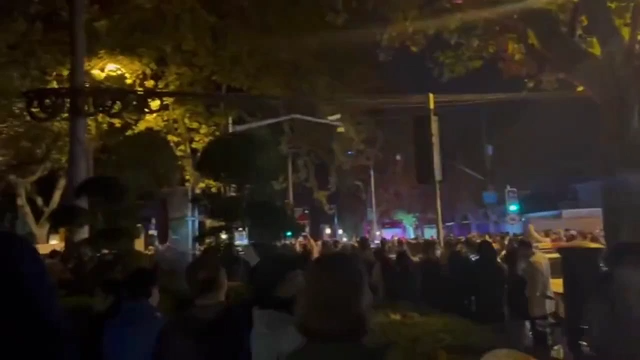
\includegraphics[width=.96\linewidth]{video_shanghai_20221126.png}}{VPlayer.swf}
	\caption{26 November 2022, Middle Urumqi Road, Shanghai}
\end{figure}
\end{frame}

\begin{frame}
Fourier transformation
\begin{equation*}
	f_k = \frac{1}{\sqrt{T}}\sum\limits_{t = 0}^{T - 1} x_t \exp(-i t {\omega}_{k})
\end{equation*}
Inverse
\begin{equation*}
	x_t = \frac{1}{\sqrt{T}}\sum\limits_{k = 0}^{T - 1} f_k \exp(i t {\omega}_{k})
\end{equation*}
Spectrum
\begin{equation*}
	s(\omega) = \frac{1}{2 \pi}\sum\limits_{k = -\infty}^{\infty} \gamma(k) e^{-i \omega k}
\end{equation*}
Every time series can be transformed to a periodogram $\Leftrightarrow$ 萬物皆輪迴
\end{frame}

%\begin{frame}{\secname}
%\begin{figure}[H]
%	\centering
%	\includegraphics[width=.8\textwidth]{}
%	\caption{}
%\end{figure}
%\end{frame}

%\begin{frame}[allowframebreaks]
%\frametitle{References}
%\nocite{*}
%\printbibliography
%\end{frame}

\end{document}